\chapter{Fast marching method} \label{chpt:fm}
Fast marching(FM) method \cite{sethian1999level} plays a very important part in both automatic neuron tracing (APP2 method) and human-guided neuron tracing. It is essentially a region-growing scheme and can be used for GSDT and initial neuron reconstruction in APP2 and finding shortest path between rays in human-guided neuron tracing.
\section{Introduction}
\subsection{Algorithm flow}
In FM, we model an image as a graph, where each graph vertex corresponds to an image pixel (voxel). There is an edge between each pair of immediately neighboring pixel-vertices. FM grows the image graph from a set of predefined seed vertices to all remaining image pixel-vertices in a distance-increasing order.  All image pixels are divided into three groups, labeled as \emph{ALIVE}, \emph{TRIAL} and \emph{FAR}. 

FM has two main steps: initialization and recursion. First, all the seed vertices are initialized to be \emph{ALIVE}; the neighbors of seeds are initialized as \emph{TRIAL}; and the rest are set as \emph{FAR}. Then, from the set of \emph{TRIAL} vertices, we will extract one vertex x, which has the minimum distance value to the \emph{ALIVE} set. The extracted vertex x is then converted from \emph{TRIAL} to \emph{ALIVE}.  For any non-\emph{ALIVE} neighbor y of x, we set it to \emph{TRIAL} if it is \emph{FAR}. The distance function of y is updated as (also see below for concrete definitions)
\begin{equation}
d(y)=min⁡{d(y),d(x)+e(x,y)}
\end{equation}

where $e(x,y)$ is the distance between vertex $x$ and vertex $y$ (see below for definition of $e(x,y)$). FM recursively extracts the vertex that has the minimum-distance from the \emph{TRIAL} set until it becomes empty.
An important implementation trick of FM is to maintain \emph{TRIAL} vertices in a Fibonacci heap so that the required minima can be obtained efficiently. See Alg.\ref{alg:fast-marching} for the algorithm flow of FM.

\begin{algorithm}[H]
\label{alg:fast-marching}
\SetKwInOut{Input}{Input}\SetKwInOut{Output}{Output}
\SetAlgoLined
\Input{seed points $x_0,x_1,\ldots,x_n$}
\Output{Return distance map $d(x)$}
Initialize distance map $d(x) = \infty$ for all point and mark as \emph{FAR} \;
Initialize $d(x_0),d(x_1),\ldots,d(x_n)$ to $0$ and mark it as \emph{ALIVE} \;
Initialize queue of \emph{TRIAL} points $Q = \O$ \;
Mark \emph{FAR} neighbors of \emph{ALIVE} points as \emph{TRIAL} (add to $Q$) and update $d$ \;
\While{Q is not empty}{
Remove minimum point $x$ from $Q$, mark $x$ as \emph{ALIVE}\;
Mark \emph{FAR} neighbors of $x$ as \emph{TRIAL} and insert into $Q$\; 
Update $d$ for the neighbors of $x$\;
}
\caption{Fast marching algorithm}
\end{algorithm}
\subsection{Min Heap}

\subsection{Differnce from dijkstra's algorithm}
In general, fast marching method is the same to Dijkstra's algorithm except that FM applys dynamic weight function. In fast marhcing method, the weight for each edge can be calculate when the edge is under marching.
\section{Applications}
Fast marching method can be applied to many bio-image processing according to the number of seed points, the definition of edge length $e(v_0,v_1)$ and the output information. The number of seed points for fast marching can be single or multiple. The edge length $e(v_0,v_1)$ can be defined as,
$$
e(v_0,v_1) = \left\{ 
    \begin{array}{lr}
    ||v_0 - v_1|| & \mbox{Euclidean distance (1)} \\
    \\
    ||v_0 - v_1|| \cdot (g_I(v_0) + g_I(v_1))/2 & \mbox{Geodesic distance (2)} \\
    \\
    ||v_0 - v_1|| \cdot (I(v_0) + I(v_1))/2 & \mbox{Image intensity (3)} \\
    \\
    f(v_0,v_1) & \mbox{other distance (4)}
    \end{array}
    \right.
$$
In the right column, $I(v)$ is image intensity at location $v$, $g_I(v)$ is expontial to image intensity $I(v)$, $f(v_0,v_1)$ is predefined distance map. The output information after fast marching may be distance map or parental map.  The related applications is classfied in tab.\ref{tab:fm-app}.\\

\begin{table}
\begin{center}
\begin{tabular}{ | c | c | c | c |}
    \hline
    \textbf{Application} & \textbf{Num of seeds} & \textbf{Edge length} & \textbf{Output} \\ \hline
    neuron reconstruction & single & geodesic distance & parental map \\ \hline
    GSDT & multiple & image intensity & distance map  \\ \hline
    3D curve drawing & multiple & geodesic distance & both \\ \hline
    Voronoi diagram & multiple & euclidean distance & parental map  \\ \hline
    seeded watershed & multiple & predefined & parental map \\ \hline
  \end{tabular}
\end{center}
\caption{This table shows some data}
\label{tab:fm-app}
\end{table}

\subsection{Shortest path for 3D curve drawing}
\label{sect:fm-3dcurve}
Draw 3D curve is a post-processing step to correct the tracing errors during automatic neuron tracing \cite{peng2011automatic, Xiao:2012}. VAA3D \cite{peng2010v3d} provides a solution to select a 3D marker by clicking mouse once or twice at most. However, it is not realistic to choose 3d markers one by one to draw a 3D curve. The convinient operation is to draw a 3D curve on 2D projection plane directly. Accuately, a drawing curve on 2D projection plane is lots of sampling lines (see Figure \ref{fig:fm-3dcurve}A) perpendicular to the projection plane. Therefore, there exist lots of potiential 3D curves corresponding to the drawing curve. To find the 3D curve (see Figure \ref{fig:fm-dynamic-drawing}B) that exactly represents the neuron segment is a tough task. Due to the narrow application, there isn't too much research about it.\\
Currently only VAA3D provides some solutions for the problem. The main idea is to use meanshift \cite{comaniciu2002mean} to estimate the 3D position for each sampling line and each meanshift estimation starts from the previous estimation position. However, for complex background noise, meanshift will fail to find the correct 3d curve (see Figure \ref{fig:fm-meanshift-drawing}B). That is because meanshift will attract to local maximum center when there exists strong background noise. To overcome the problem, it is needed to define a global optimaized model by considering all internal sampling lines. \\
\subsubsection{Shortest path model}
Shortest path provide a good model for choosing the best 3d curve. The model assumes that the expected 3d curve is the shortest path by accrossing all the internal sampling lines including the first and last sampling lines. The length between consective vertices (or points) $v_0$ and $v_1$ is defined as, 
$$
e(v_0,v_1) = ||v_0 - v_1||\cdot \left( \frac{g_I(v_0) + g_I(v_1)}{2} \right)
$$
which is the geodestic distance widely used in neuron tracing \cite{peng2010automatic, peng2011automatic}. $g_I(v_i)$ on the right item is defined as ,
$$
g_I(v_i) = exp(\lambda_I(1-I(v_i)/I_{max})^2)
$$
where $I(v_i)$ is the intensity of vertex $v_i$ and $I_{max}$ is the maximum intensity of the entire image $I$. So the edge length between bright points will be very small, which ensure the shortest path go accross the continuous bright points as much as possible.
For the proposed model, there are two problems needed to sovle. First, find all shortest paths from subject line to all vertices on the target line. Second, find the global shortest path accrossing all internal lines.
\subsubsection{Find all shortest paths}
In this step, we need to find the shortest path from the subject line to each vertex on the target line. This problem can be perfectly sovled by fastmarching method. Firstly, all the vertices on the subject line will be used as seed points. Then marching from the seed points until all vertices on the target line are marched. From the resulting distance tree, we can easily get the shortest path by reverse from each vertex on the target line until the first vertex on the source line is visited. In practice, there is no need to march all vertices on the target line; normally when 50\% vertices are marched, the marching process can stop.\\
This problem is the extension of finding the shortest path between two lines. And it is not restricted to lines, any two groups of points can find the shortest path by using fastmarching method.
\subsubsection{Find global shortest path}
After finding all shortest path between first and second line, we can get the shortest marching distance for the vertex on second line. This value can be used to initialize $\phi(v)$ when the second line march to third line to find all the shortest path. Actually, the resulting shortest path is the shortest path from first line to vertices on third line by accrossing some vertex on second line. Continusly finding the shortest paths, we will find all shortest paths from the first line to the last line by accrossing all internal lines. We just need to choose the path, which firstly reach the last line, as the final 3D curve (see model on Figure \ref{fig:fm-dynamic-compare}A and result on Figure \ref{fig:fm-dynamic-drawing}C).
\subsubsection{Further optimization}
The global optimized result is not always good when the sampling line deviated to background (see Figure \ref{fig:fm-dynamic-compare}C). Actually, the sampling line should be used as a reference to indicate that the 3D curve should near to the line. For consective lines, we can set a bounding box. So we can change the model as the 3D curve is the shortest path from the first line to the last line by accrossing the boudingboxes between consective lines (see Figure \ref{fig:fm-dynamic-compare}B). We can see the different drawing results with same sampling lines, Fig.\ref{fig:fm-dynamic-compare}C for original model and Fig.\ref{fig:fm-dynamic-compare}D for improved model. The original model may produce lots of spurs near sampline lines while the impoved model produces much smoother result.
%\includegraphics{2_dynamic.pdf}

\begin{figure}[htb]
\begin{center}
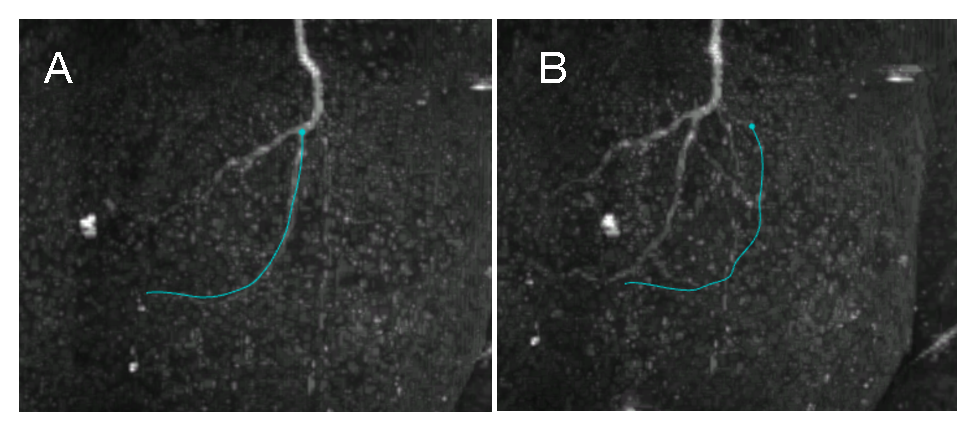
\includegraphics[width=5in]{images/fm_meanshift_drawing}
\caption{(A) meanshift based curve drawing. (B) error occured on noisy background}
\label{fig:fm-meanshift-drawing} % \lable should be after \caption
\end{center}
\end{figure}

\begin{figure}[htb]
\begin{center}
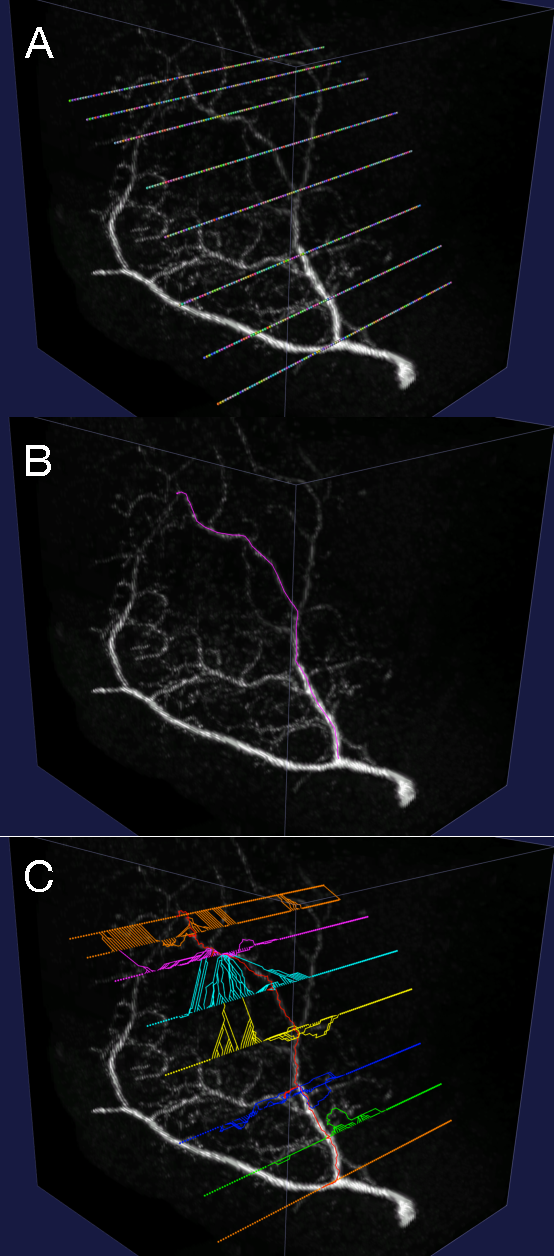
\includegraphics[width=6in]{images/fm_dynamic_drawing}
\caption{(A) sampling lines. (B) expected 3D curve. (C) the process of global optimized model}
\label{fig:fm-dynamic-drawing}
\end{center}
\end{figure}

\begin{figure}[htb]
\begin{center}
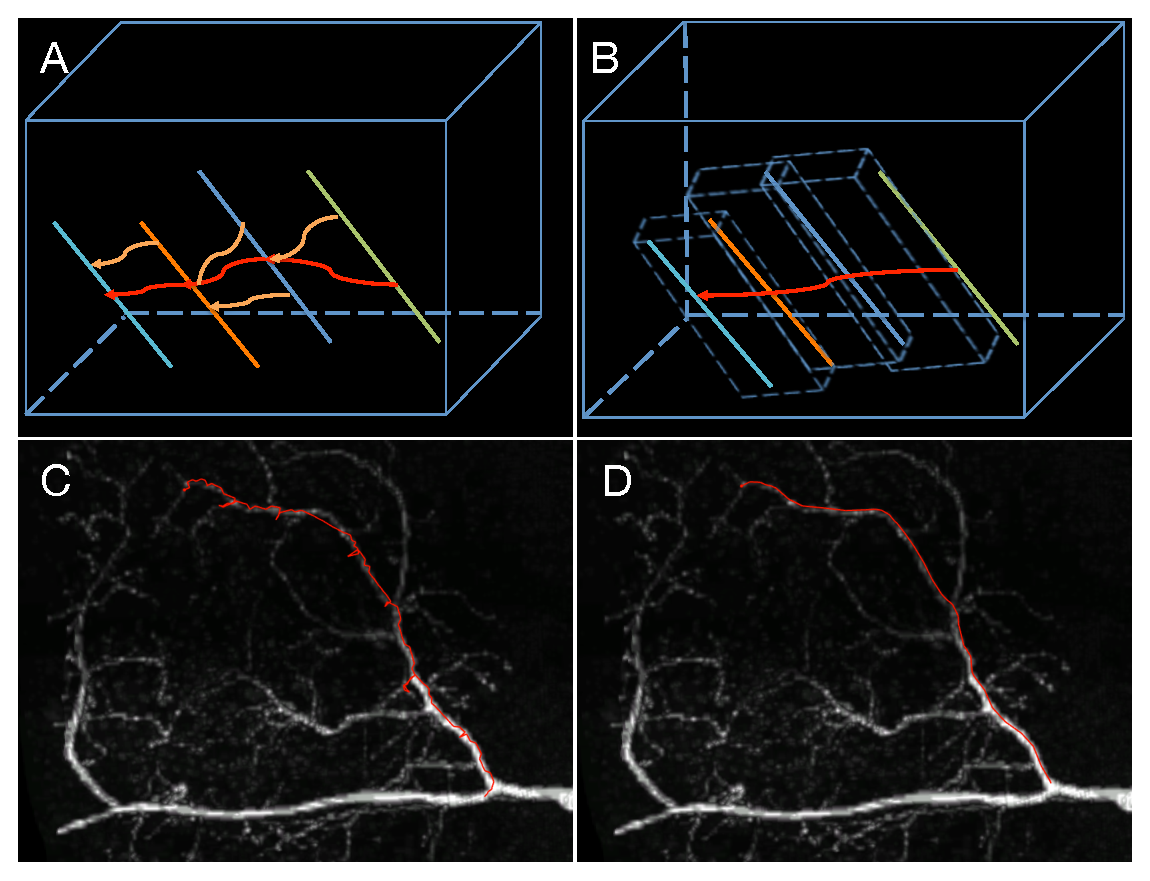
\includegraphics[width=5in]{images/fm_dynamic_compare}
\caption{(A) global optimized model. (B) improved bounding-box model (C) the result or original model. (D) the result of improved model}
\label{fig:fm-dynamic-compare}
\end{center}
\end{figure}
\subsection{Gray-weighted distance transfrom}
\subsection{Generalized Voronoi diagram for shapes} \label{subsec:gvd}
In image processing, a Voronoi diagram \cite{aurenhammer1991Voronoi} is a special kind of decomposition of an image, determined by distances to a group of specified objects. These objects can be many seed points (Figure \ref{fig:fm-Voronoi}A) normally or many cell bodies (Figure \ref{fig:fm-Voronoi}B). The Voronoi Diagram for cell bodies is also called Generalized Voronoi Diagram (GVD) \cite{nath2007accurate}. The decomposted image areas are Voronoi areas. Each Voronoi area is a group of points whose nearest object are the same. Voronoi Diagram can be found in a large number of fields in science and technology, even in art.\\
There are lots of algorithms proposed to solve the Normal Voronoi Diagram. Lloyd \cite{lloyd1977triangulations} firstly consider the problem as a k-means clustering problem. A more efficent algorithm for generating a Voronoi Diagram in a plane is proposed by Fortune \cite{fortune1987sweepline} in $O(nlog(n))$ time. The method need to scan the image from left to right with a sweep line. For higher dimension image, Bowyer Watson \cite{rebay1993efficient} proposed a method to solve the complementary problem Delaunay triangulation in any number of dimensions. However, these algorithms only solve the Normal Voronoi Diagram problem. For the Generalized Voronoi Diagram problem, there isn't efficient methods \cite{hoff1999fast, takahashi1989motion, nath2007accurate}. Actually either normal Voronoi diagram or generalized Voronoi diagram problems can be considered as a shortest path problem by growing seed points or cell bodies to nearest area. It is a fast marching problem. The only thing we need to do is labeling each object with unique lable. Each pixel will be labeled the same to its nearest object.

\begin{figure}[htb]
\begin{center}
\includegraphics[width=4in]{images/fm_Voronoi}
\caption[Normal Voronoi diagram and generalized Voronoi diagram]{(A) sampling lines. (B) expected 3D curve. (C) the process of global optimized model}
\label{fig:fm-Voronoi}
\end{center}
\end{figure}
